%%%%%%%%%%%%%%%%%% Latex %%%%%%%%%%%%%%%%%%%%%
\documentclass[12pt]{article}

\usepackage{amsmath}
\usepackage{shadow}
\usepackage{dingbat}
%\usepackage{wasysym}
%\usepackage{bbold}
\usepackage{amssymb}
\usepackage{slashed}
%\usepackage{graphics}
\usepackage{graphicx}
%\usepackage{pstricks,pst-node,pst-tree}
\usepackage{fancybox}

% equations
\def\TT{{\mathrm TT}}
\def\N{{\cal N}}
\def\GG{{\cal G\hspace{-2.3mm}G}}
\def\Gg{\mathbb G}
\def\E{{\cal E}}
\def\B{{\cal B}}
\def\lrd{\stackrel{\leftrightarrow}{\partial}}

\def\chib{\overline\chi}
\def\psib{\overline\psi\hspace{-2.6mm}\phantom{\psi}}
\def\tid{\hspace{.3mm}}
\def\ve{\varepsilon}
\def\D{{\cal D}}
\def\M{{\cal M}}
\def\J{{\cal J}}
%greek
\def\a{\alpha}
\def\b{\beta}
\def\de{\delta} 
\def\De{\Delta}
\def\eps{\epsilon}
\def\r{\rho}
\def\k{\kappa}
\def\l{\lambda}
\def\m{\mu}
\def\n{\nu}
\def\s{\sigma}
\def\t{\tau}
\def\z{\zeta}


%phantoms
\def\ph#1{\phantom{#1}}
\def\ag#1{\gamma({\scriptstyle #1})}
\def\Sl#1{\slashed{#1}}
%\def\Sl#1{#1\hspace{.1mm}\!\!\!\!/\,}
\def\sl#1{\slashed{#1}}
\def\wh#1{\widehat{#1}}
\def\wt#1{\widetilde{#1}}
\def\mt{{\tilde \mu}}
\def\nt{{\tilde \nu}}
\def\rt{{\tilde \rho}}
\def\st{{\tilde \sigma}}
\def\ol#1{\overline{#1}} 
\def\sss{\scriptscriptstyle}
\def\ts{\textstyle}
\def\d{{\bfseries d}}
\def\la{\langle}
\def\ra{\rangle}
\def\e{\epsilon}
\def\scirc{\!{\scriptstyle \circ}}
\def\psitb{\overline{\widetilde\psi}}
\def\vphi{\varphi}
\def\psid{\psi^\dagger}

%Sets
\def\F{{\cal F}}
\def\O{{\cal O}}
\def\Z{{\mathbb{Z}}}
\def\Q{{\mathbb{Q}}}
\def\A{{\mathbb{A}}}
\def\R{{\mathbb{R}}}
\def\C{{\mathbb{C}}}
\def\H{{\mathbb{H}}}

%\matricies
\def\ba{\left(\begin{array}{cc}}
\def\ea{\end{array}\right) }
\def\be{\begin{equation}}
\def\ee{\end{equation}}
\def\beq{\begin{equation}}
\def\eeq{\end{equation}}
\def\bea{\begin{align}}
\def\eea{\end{align}} 
\def\beqa{\begin{equation}\begin{array}{l}}
\def\eeqa{\end{array}\end{equation}}

%--------------------------------------------
% symbols
%warning \be is for equations now
\def\ga{\gamma} 
\def\G{{\it\Gamma}} 
\def\g{\gamma}
\def\veps{\varepsilon}  
\def\L{{\it\Lambda}}
\def\Pit{{\it\Pi}}
\def\Psit{{\it\Psi}}
\def\si{\sigma} \def\Si{{\it\Sigma}}
\def\th{\theta} \def\vth{\vartheta} \def\Th{\Theta}
\def\w{\omega} \def\W{\Omega} \def\hw{\hat{\omega}}
\def\vfi{\varphi}\def\vphi{\varphi}
\def\bra{\langle} \def\ket{\rangle}
\def\dd{{\mathrm d}}
\def\pa{\partial}
\def\vrho{\varrho}

\def\ie{{i.e., }}
\def\eg{{e.g.\ }}
\def\LR{\Leftrightarrow} 
\def\cl{\centerline}

\def\pa{\partial}
\def\rarr{\rightarrow}
\def\nn{\nonumber}

\def\psibar{\overline{\psi}}
\def\Gbar{\overline{G}}

\def\psidag{\psi^\dagger}
\def\Gdag{G^\dagger}

\def\N{{\bfseries N}\,}
\def\TR{{\bfseries tr}\,}
\def\G{{\bfseries g}\,}
\def\DIV{{\bfseries div}\,}
\def\GRAD{{\bfseries grad}\,}
\def\ord{{\bfseries ord}\,}

\def\Nt{{\cal N}}
\def\Tt{{\cal T}}
\def\c{{\hspace{.3mm}\bfseries c\hspace{.3mm}}}
\def\Real{\mathbb R}

\def\noi{\noindent}

\def\thup{\rightthumbsup}
\def\thdn{\rightthumbsdown}

%\def\checkmark{\tikz\fill[scale=0.4](0,.35) -- (.25,0) -- (1,.7) -- (.25,.15) -- cycle;}

%%%%%%%%%%%%%%%%%%%%%%%%%%%%%%%%%%%%%%%%%%%%

\begin{document}

\thispagestyle{empty}
~
\vspace{-3.9cm}
\begin{center}
{
\Large
 {\bfseries  Writing With Mathematics \\
 Part II: Words and Statements }  \\[10mm]
 {  
 \vspace{-.9cm} 
%MAT 003-03, SMC Fall, 2013\\
Cherney}\\[1mm]
%{\small Office hours: Tues \& Thurs 2-4pm, Galileo 103A\\dmc13@stmarys-ca.edu}
\vspace{3.5mm}
}

\end{center}
\

%\section{The Basics of Writing With Math} 

The most basic thing to understand about writing with math is that math is not some collection of symbols unrelated to the tools you write with (roman letters and punctuation) but rather part of that language. Excessive emphasis on scratch-work style calculations leads many people to believe otherwise, but go back and look at any textbook you have used, wikipedia articles, scholarly writing etc, and you will see that this is erroneous thinking. If you wish to communicate in written form about the math you have learned you must learn to treat mathematical symbols as an extension of your language, not as a disjoint language. 

\section{Expressions are Nouns.\\ Equations are Statements.}
The string of words ``2+3" is a noun. 
It can be used as the subject of a sentence such as ``$2+3=5.$" 
Compare this to the noun ``Josh and Liz" and the sentence ``Josh and Liz are friends." 
Algebraic expressions are also nouns. For example ``3x+2y" is a noun.  An algebraic equation such as ``3x+2y=5." is a sentence. 

Complex sentences can be built by using  equations, inequalities, etc as clauses. 
The following sentence does so. 
``If $3x-2=7$ then $3x=9$ and therefore $x=3$."
\\





\subsection{Diagrams are not words}
The following is a writing mistake that comes from not recognizing this fact.\\

\shabox{
The graph 
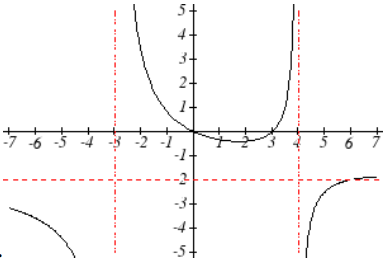
\includegraphics[height=2.8cm]{rat}
has a vertical asymptote at 3.} \thdn \\

\noi To remedy this, simply construct a sentence that makes reference to your diagram as in the following.\\

\shabox{
The graph drawn below has a vertical asymptote at 3.\\[.1cm]
\phantom{The graph drawn} 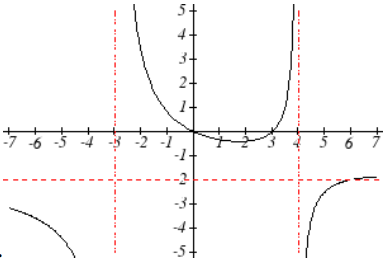
\includegraphics[height=3cm]{rat} } \thup\\

Certainly diagrams play an important  role in communication, but when writing one ought to be clear about what is verbal and what is diagrammatic. Notice, in particular, that mathematical shorthand like ``$f:A\to B$ is {\it not}" diagrammatic but rather shorthand. 

%Make it clear where a line begins and ends.\\

\subsection{Math Notation is shorthand, and then some}

The string of symbols ``$3(2+1)=9$" is shorthand for ``three times two plus one is equal to nine." The old Arabic symbols ``$0$",``$1$",$\dots$,%2,3,4,5,6,7,8,
and ``$9$"  have become a standard shorthand for the words ``zero", ``one" et cetera. Likewise, the symbol ``=" has become shorthand for the words ``is equal to". \\

%\noi (If my use of quote marks  confuses you, look up ``use-mention distinction".)\\


Unfortunately the string of words ``three times two plus one" is ambiguous; it can be interpreted as $3\cdot2+1$ or $3(2+1)$. The ambiguity can be cleared up by elongating the string of words to ``the result of first summing two and one and then multiplying the result by three". 
This is tedious to read or write. The parentheses in ``$3(2+1)$" serve as a shorthand for specifying which operations are to be performed first. One can only imagine how much paper has been saved by using arabic numerals and parentheses (along with shorthand for the operations addition, subtraction, multiplication, division, exponentiation, et alia) as shorthand. Our society has benefitted tremendously from the development of these notations, and you are expected to learn to read and write them accurately. You can invent your own notations (legend has it Einstein said that his greatest contribution to science was good notation, and yours could be better than his!) but if you are using anything other than standard notations, you need to tell your audience exactly how to read it! 

%There are standard shorthand symbols. 
%As with grammar, don't invent your own conventions.\\
Probably the most misused notation is the arrow symbol. 
In the most widespread convention,  ``$\to$" is shorthand for ``goes to" (a common phrase in calculus and analysis) while ``$\implies$" is shorthand for ``implies". A good example of using the latter symbol is the following sentence. 
\begin{quote}
\shabox{$x+1=2 \implies x=1.$} \thup
\end{quote}
You just read shorthand for ``The algebraic equation $x$ plus one is equal to two implies the algebraic equation $x$ is equal to one." 

It is important to note that the terms ``implies" and ``is equal to" are very different! The following exemplifies a common mistake that comes from not recognizing this distinction.
\begin{quote}
\shabox{$x+1=2 = x=1.$} { \thdn}
\end{quote}
Read as written this says ``x plus one is equal to two which is equal to x which is equal to one." Part of what is being said in the sentence is $1=2$. It is rare that someone wishes to communicate this idea.

Many texts and instructors use ``$\to$" as shorthand for ``implies", but in this class we will follow the more common convention. To be clear look at this awkward example; we will read 
%\begin{quote}
``$x+1=2 \to x=1.$" as ``$x$ plus 1 is equal to two goes to $x$ is equal to one." If you wish to convey this idea you need to specify the process by which one equation becomes the other. 
%\end{quote}
%e.g. $\to$ all overs the place.\\
%$=$ vs $\implies$ vs 

The symbol $\Leftrightarrow$ is shorthand for ``is equivalent to" and can be used when modifying algebraic equalities or inequalities. An example of correct use of this term is the following sentence. 
\begin{quote}
\shabox{$x+1=2 \LR x=1.$} \thup
\end{quote}
An incorrect use of this term is the next sentence.
\begin{quote}
\shabox{$x>2 \LR x>1.$} \thdn
\end{quote}
The reason this is incorrect is that while $x>2 \implies x>1$ it is not the case that $x>1 \implies x>2.$



\section{Technical Vocabulary Facilitates Concision }

The idea of a definition of a word should perhaps be split into two ideas. \\

Consider the word `gross' and all of its various meanings. 
The word has thousands of years of history and for most of that time no one learned the word by looking up a definition in a dictionary. The meaning of the word developed organically from prehistory to today through millions of uses and perceived misuses. Each of us have been exposed to some of those uses and that is how we learned the word. 
To write the entire history of the word, each of its uses throughout history and all of the connotations and connections involved, would be impracticable. 
Dictionary entries for the word `gross' aim to consolidate descriptions of all of those uses. This is the kind of definition one encounters most often: definitions that are {\it descriptive}.

{\it Prescriptive } definitions, by contrast, are often given in mathematics (and other technical fields). An example is given below. \\

 \noi
 {\bfseries Definition}: An algebraic equation is {\bfseries trivial} (or {\bfseries tautological}) if substitution of any number(s) for its variable(s) yields a true arithmetic statement. \\

This definition does not aim to summarize how the word has been used in the past. It is a declaration that the word will be used to convey this meaning and nothing more. (At least in the particular book, paper, course etc in which the definition is given.) These prescriptive definitions are not organic. 
They are intentionally created and intentionally presented to achieve a specific purpose. 
That purpose is typically to facilitate concise statements of fact. 
Take for example the following statement.
\begin{quote}
If a function is differentiable on the interval $(a,b)$ then it is continuous on the interval $(a,b)$.
\end{quote}

\noi This is surely more concise than the following equivalent statement that does not use the technical terms {\it differentiable} and  {\it continuous} but rather their prescribed meanings. 

\begin{quote}
If a function $f$ has the property that the two sided limit 
\[\lim_{h\to0}\frac{f(c+h)-f(c)}{h} \] exists for all numbers $c$ in the interval $(a,b)$ then 
it also has the property that the two sided limit \[\lim_{x\to c} f(x)\] exists for all values of $c$ in the interval $(a,b)$.
\end{quote}

Professional mathematicians build prescriptive definitions such that many relationships between the defined objects can be deductively proven. This building of definitions and proving of statements happens in small communities, and only a few people (math PhDs) witness the process. When a community builds a powerful and useful collection of definitions and proofs, relevant communities of non-mathematicians are made aware. %That is one way to describe what mathematicians do: develop useful prescriptive definitions and powerful theorems within mathematical communities.

You, dear student, are in one of those relevant communities of non-mathematics: the community of engineering, physics, chemistry, etc majors. But the difference in kinds of definitions (descriptive and prescriptive) is rarely made clear to students. The result is often confused (and confusing) use of technical terms. I've collected some below.  For the prescriptive definitions of terms used see the handout  Terminology from Elementary Algebra.\\




\shabox{Consider the curve $y=x^2$.} \thdn \\

\shabox{Consider the solution set to the algebraic equation $y=x^2$.}\thup\\

\noi The solution set to that equation is a parabola. \\


\shabox{\noi The function $f$ is $y=3x$.} \thdn \\

\shabox{\noi The %rule of correspondence of the 
function $f$ assigns the number $3x$ to any $x$ in the domain of $f$.} \thup \\

\noi Functions are not equations.\\

\shabox{\noi The equation $3x+1$ is linear.}\thdn \\

\shabox{\noi The function $3x$ is linear.}\thup \\

\shabox{\noi The equation $y=3x+1$ is linear.}\thup \\

\noi Algebraic expressions are not algebraic equations.\\

\shabox{\noi If $f(x)=x+1$ then the function $f(1)=2$.} \thdn\\

\shabox{\noi If $f(x)=x+1$ for all numbers $x$ then $f(1)=2$.} \thup\\

\noi 
If a function is named $f$ then neither the expression $f(x)$ nor $f(1)$ is a function. They are the value assigned to $x$ and the value assigned to $1$ by f, respectively. \\



\shabox{\noi If the domain of $f$ is $[0,3)$ then the function $f(4)$ is not defined.}\thdn \\

\shabox{\noi If the domain of $f$ is $[0,3)$ then $f(4)$ is not defined.}\thup \\

Again if $f$ is a function then $f(4)$ is not a function. \\



\shabox{\noi When one derives $x^2$ one obtains $2x$.} \thdn\\

\shabox{\noi The derivative of $x^2$ is $2x$.} \thup\\

\noi The verb meaning `to calculate the derivative of' is differentiate, not derive. \\






\subsection{Category Errors}
These uses can often be described as {\it category errors}. A category error is assigning a property to an object that can not possibly have that property. For example, my computer is not angry despite the evidence; it crashes every time I play my favorite video game. Computers can not have the property of anger. They are not in the category of things that can be angry.

\shabox{\noi If $f(x)=x^2$ then  $(2,4)$ is solution to the function.} \thdn \\

\shabox{\noi If $f(x)=x^2$ then $(2,4)$ is in the graph of $f$. } \thup \\

\noi Functions do not have solutions and algebraic equations do not have graphs. \\


\shabox{\noi To find a  solution to the system of equations 
\[y=2x-1\]
\[y=x+1\]
set the equations equal to each other.}\thdn \\

\shabox{\noi To find a  solution to the system of equations 
\[y=2x-1\]
\[y=x+1\]
one may substitute the right hand side of the first for $y$ in the second to obtain
\[
2x-1=x+1
.\]}\thup \\

\noi A pair of functions can not have the property that the equations are equal; 
$(y=2x-1)=(y=x+1)$ is a meaningless statement. \\


%



These examples may seem pedantic to you, and you could probably find textbooks that make many of these mistakes that you have been able to read  comfortably. 
There is good reason for so-called abuse of notation; you probably noticed that some of the thumb up examples above were considerably longer than the corresponding thumb down examples. However, the author of this note has found these points of confusion to be the most common causes of incomprehensible writing with mathematics. 
It is hoped that explicitly pointing these things out once will help the reader make better informed choices for her writing in the future.  



\section{Pronoun Ambiguity and Overuse}

When one is not yet fluent in a technical language one has a tendency to recall technical terms too slowly to incorporate them into what is being said. This leads one to use pronouns instead of nouns.

\begin{center}
\shabox{
%\[
%\bv 1\\1\ev,  
%\bv 1\\2 \ev, 
%\bv  0\\1\ev
%\] are vectors and 
If you subtract it from it you get it. }\thdn
\end{center}

Remember, every time you use a pronoun you are expecting your reader to read your mind; the meaning of pronouns needs to be clear from the context. In particular, using the same pronoun (like ``it") for several different nouns in the same sentence is almost always confusing. 

\section{Say what your symbols mean}
The following statement is false if  $n=\frac12$.
\begin{center}
\shabox{
For all $n$ the number $2n$ is even.
}\thdn
\end{center}
When you use a symbol to stand for any element of a collection of object, let your reader know what collection of objects you have in mind. 
\begin{center}
\shabox{
For any integers $n$ the number $2n$ is even.
}\thup
\end{center}
This becomes especially important in higher level math classes where set of objects besides real numbers or integers are common; a symbol may stand for a function, vector, linear operator, matrix, etc.

\subsection{Particular, Arbitrary, or General?}

In mathematics writing you commonly encounter these three words, and it can be difficult to sort out their meanings.

The word ``particular" points out just one object
\begin{center}
\shabox{
The sum $\sum\limits_{k=0}^n n^2= \frac{n(n+1)(2n+1)}{6}$ for a particular $n$. 
}\thdn
\end{center}
While the statement is true since the equality is try with n replaced by $1$, it is likely that the author of this statement intended to convey that the equality with $n$ replaced by any natural number. (I only wrote ``the sum" at the beginning of this sentence to avoid beginning a sentence with shorthand notation. Doing so is considered bad form.)
\begin{center}
\shabox{
The sum $\sum\limits_{k=0}^n n^2= \frac{n(n+1)(2n+1)}{6}$ for an arbitrary natural number $n$. 
}\thup
\end{center}

The word ``arbitrary" is used to point out that a statement is true if a symbol within it is replaced with any particular member of a set.

\begin{center}
\shabox{
The equality $3x+1=4$ is true for a particular real number $x$.}\thup
\end{center}


The word ``general" is used outside of mathematics to say that a statement is true more often then not. But it is not used that way in mathematics.

\begin{center}
\shabox{
If you are being rained upon, then there is generally a cloud above you.}~\thdn
\end{center}
Sometimes the sky is blue just above you, but wind blows rain onto you. In mathematics, the word ``general" conveys that a statement is always true. \\


\shabox{
The numbers $12$ and $14$ can be expressed as  $3\cdot2\cdot2$ and $2\cdot 7$, respectively. In general, if $n$ is a natural number then 
$n$ can be expressed as the product of prime numbers.}~\thup

%\subsection{Unknown, variable, or arbitrary constant?}








\section{Recap}
\begin{itemize}

\item Mathematics is not a separate written language. 
\item Expressions and equations are grammatical structures. 
\item Mathematics utilizes considerable shorthand notation, but the symbols used are not diagrams. 
\item Diagrams and pictures are not words.
\item Math uses prescriptive definitions. The resulting technical vocabulary is a central part of what you are meant to learn in a math course. 
\end{itemize}
%\section{Categorical error}
%
%The data set is linear. \\
%
%The graph of the equation.\\
%
%The solution of the function. \\
%
%The domain of the equation. \\





%Parenthese. 



%\section{Your Audience}
%Write for your audience. \\
%Don't copy the wording of problems you have been given. \\
%Give sufficient context.\\
%Show calculations in a readable way.\\
%Don't show every detail. (e.g. of arithmetic)\\
%
%Writing for a professor is extremely weird; your prof has seen so many mistakes that, by assuming you are making the usual mistakes, he can read your mind when your writing would be incomprehensible to any other kind of person. 
%Pretend your audience is a classmate that has not read the question/problem recently. 
%%It may very well be. \\
%You should never have to say ``you know what I mean", you should always say what you mean.







\end{document}

